\section{Results and Discussion} \label{sec:results}

\subsection{Phylometric Signatures of Evolutionary Dynamics}

\begin{teaserfigure}
  \centering
  % \begin{noindent}
  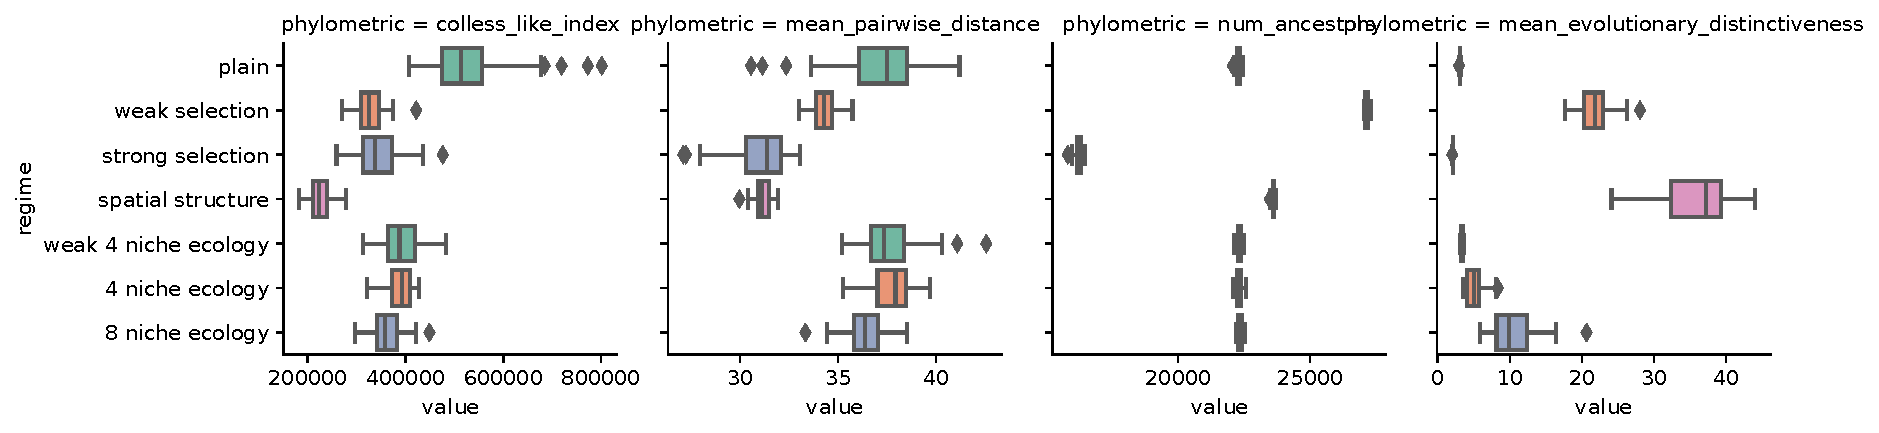
\includegraphics[width=\textwidth]{binder/binder/teeplots/col=phylometric+epoch=7+mut_distn=np.random.standard_normal+viz=boxplot+x=value+y=regime+ext=.pdf}
  % \end{noindent}
  \caption{%
    Distribution of phylometrics measured with perfect phylogenetic tracking across surveyed evolutionary regimes ($n=50$).
  }
  \label{fig:perfect-tree-phylometrics}
\end{teaserfigure}


The feasibility of harnessing phylogenetic analysis to characterize evolutionary dynamics in digital evolution systems hinges on the premise that these dynamics induce detectable structure within the phylogenetic record.
In order to explore this tenet, we compared distributions of phylogenetic metrics yielded across replicate runs under different sets of evolutionary conditions. Figure \ref{fig:perfect-tree-phylometrics} summarizes these distributions.  Indeed, statistical tests confirmed that each phylometric exhibited significant  variation among surveyed evolutionary conditions (Kruskal-Wallis tests; all $p < 1\times10^{-50}$; $n=50$ per condition; Supplementary Table tab:perfect-tree-phylometrics-kruskal).

To better understand, we performed an all-pairs comparison of each phylometric among the seven surveyed evolutionary regimes (Wilcoxon tests with Bonferoni correction; corrected significance thresh $1.49 \times 10^{-4}$; $n=50$ per condition; 84 comparisons per sensitivity analysis configuration; 336 comparisons total; Supplementary Table tab:perfect-tree-phylometrics-wilcox).

 The Colless-like index is significantly depressed under all evolutionary regimes compared to the plain regime with no spatial structure, no ecology,  and moderate selection pressure.
This indicates that all deviations from baseline conditions increased regularity in generated phylogenies.
% TODO this is counterintuitive and counter to expectations; come up with a plausible explanation and commentary

Compared to the plain regime, observed mean pairwise distance was significantly lower under strong selection and significantly higher under weak selection and with spatial structure.
None of the ecological regimes induced significant changes in the mean pairwise distance phylometric compared to the plain regime.

Similarly, ancestor account had no significant relationship with ecology. However, weak selection and spatial structure significantly increased ancestor count and strong selection significantly decreased it.

Finally, mean evolutionary distinctiveness was significantly increased under all three ecological regimes compared to baseline.
Additional, ecological intensity was significantly associated with mean evolutionary distinctiveness, with weak 4 niche ecology having the lowest value for this phylometric and 8 niche ecology having the highest.
However, evolutionary distinctiveness was more strongly driven by weak selection and even more strongly driven by spatial structure, by significant margins.
Finally, strong selection significantly depressed mean evolutionary distinctiveness. 

\begin{teaserfigure}
  \centering
  % \begin{noindent}
  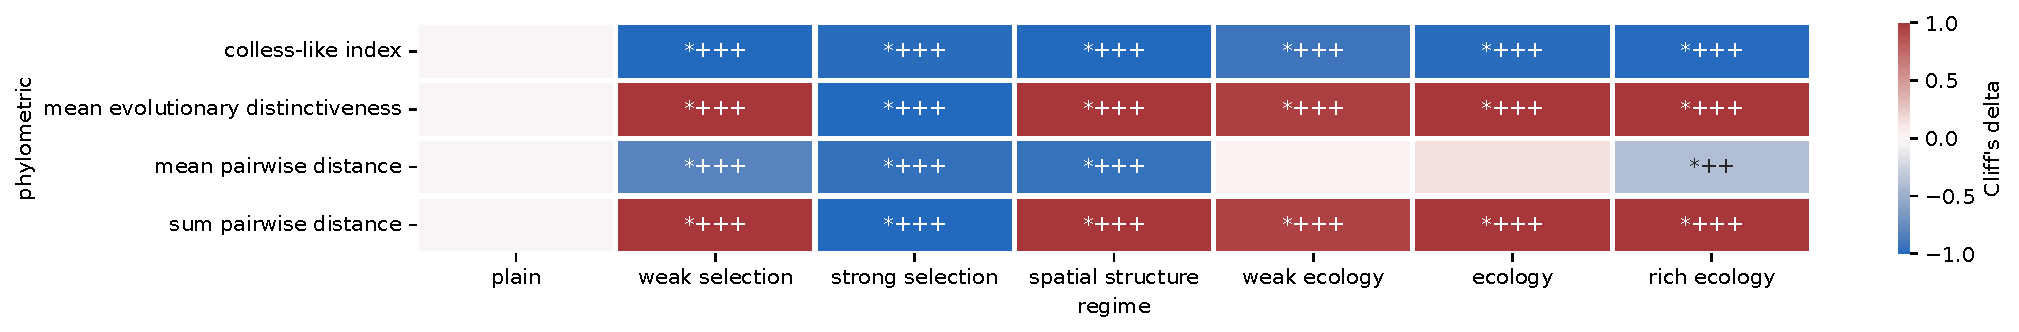
\includegraphics[width=\textwidth]{binder/binder/teeplots/epoch=7+mut_distn=np.random.standard_normal+viz=heatmap+x=regime+y=phylometric+ext=.pdf}
  % \end{noindent}
  \caption{%
    Phylogenetic metric values across surveyed evolutionary conditions, relative to plain regime.
  }
  \label{fig:perfect-tree-phylometrics}
\end{teaserfigure}


Figure \ref{fig:perfect-tree-phylometrics-heatmap} provides a high-level overview of the magnitude and direction of each regime's effects on evolutionary metrics compared to the plain regime.
Notably, strong and weak selection both significantly decrease Colless-like index and mean pairwise distance but have opposite effects on ancestor count and mean evolutionary distinctiveness.
Colless-like distance appears to be the least useful metric in distinguishing evolutionary dynamics, decreasing under all non-plain evolutionary conditions.

Ecological dynamics have significant, but relatively weak, influence on the surveyed phylometrics.
So, it appears careful accounting for other evolutionary dynamics (i.e., selection pressure and spatial structure) will be essential to accurate detection of ecology through phylogenetic analysis.
Ancestor count and mean pairwise distance may play a role in identifying ecological dynamics, as ecological dynamics --- in contrast to other factors such as spatial structure and changes in selection pressure --- have little to no discernible effect on these phylometrics. 
Alternately, in future work it may be possible to develop phylometrics that respond more strongly --- and more exclusively --- to ecological dynamics.

We performed a sensitivity analysis over an alternate exponential mutation operator and earlier phylogeny sampling timepoints.
We found the effects of evolutionary conditions on phylometrics to be generally consistent across surveyed conditions (Supplementary Figures \ref{fig:perfect-tree-phylometrics-sensitivity-analysis} and \ref{fig:perfect-tree-phylometrics-heatmap-sensitivity-analysis}; Supplementary Tables tab:perfect-tree-phylometrics-kruskal and tab:perfect-tree-phylometrics-wilcox). 

% results at epoch 7
%     \begin{itemize}
%         \item plain	4 niche ecology	50	mean pairwise distance
%         \item plain	4 niche ecology	50	num ancestors
%         \item plain	8 niche ecology	50
%         \item mean pairwise distance
%         \item plain	8 niche ecology	50	num ancestors
%         \item strong selection	8 niche ecology	50 colless like index
%         \item strong selection	spatial structure	50	mean pairwise distance
%         \item weak 4 niche ecology	4 niche ecology	50	colless like index
%         \item weak 4 niche ecology	4 niche ecology	50	mean pairwise distance
%         \item weak 4 niche ecology	4 niche ecology	50	num ancestors
%         \item weak 4 niche ecology	8 niche ecology	50	num ancestors
%         \item weak 4 niche ecology	plain	50	mean pairwise distance
%         \item weak 4 niche ecology	plain	50	num ancestors
%         \item weak selection	strong selection	50	colless like index
%     \end{itemize}

% results at epoch 0
% \begin{itemize}
% \item 4 niche ecology	weak 4 niche ecology	50	colless like index
% \item 4 niche ecology	weak 4 niche ecology	50	mean pairwise distance
% \item 4 niche ecology	weak 4 niche ecology	50	num ancestors
% \item 8 niche ecology	4 niche ecology	50	num ancestors
% \item 8 niche ecology	weak 4 niche ecology	50	num ancestors
% \item plain	4 niche ecology	50	mean pairwise distance
% \item plain	4 niche ecology	50	num ancestors
% \item plain	8 niche ecology	50
% \item mean pairwise distance
% \item plain	8 niche ecology	50	num ancestors
% \item plain	weak 4 niche ecology	50	mean pairwise distance
% \item plain	weak 4 niche ecology	50	num ancestors
% \item spatial structure	weak selection	50	mean evolutionary distinctiveness
% \item strong selection	4 niche ecology	50	colless like index
% \item strong selection	8 niche ecology	50	colless like index

% \end{itemize}

% results at epoch 2
% \begin{itemize}
%     \item 8 niche ecology	4 niche ecology	50	num ancestors
%     \item 8 niche ecology	weak 4 niche ecology	50	num ancestors
%     \item plain	4 niche ecology	50	mean pairwise distance
%     \item plain	4 niche ecology	50	num ancestors
%     \item plain	8 niche ecology	50	mean pairwise distance
%     \item plain	weak 4 niche ecology	50	mean pairwise distance
%     \item plain	weak 4 niche ecology	50	num ancestors
%     \item strong selection	8 niche ecology	50	colless like index
% \item strong selection	spatial structure	50	mean pairwise distance
% \item weak 4 niche ecology	4 niche ecology	50	colless like index
% \item weak 4 niche ecology	4 niche ecology	50	mean pairwise distance
% \item weak 4 niche ecology	4 niche ecology	50	num ancestors
% \item weak selection	strong selection	50	colless like index

% \end{itemize}

% results at epoch 7, exponential
%     \begin{itemize}
%         \item 4 niche ecology	8 niche ecology	50	colless like index
%         \item 4 niche ecology	8 niche ecology	50	num ancestors
%         \item 4 niche ecology	weak 4 niche ecology	50	colless like index
%         \item 4 niche ecology	weak 4 niche ecology	50	mean pairwise distance
%         \item 4 niche ecology	weak 4 niche ecology	50	num ancestors
%         \item plain	4 niche ecology	50	mean pairwise distance
%         \item plain	4 niche ecology	50	num ancestors
%         \item plain	8 niche ecology	50	mean pairwise distance
%         \item plain	weak 4 niche ecology	50	mean pairwise distance
%         \item plain	weak 4 niche ecology	50	num ancestors
%         \item weak 4 niche ecology	8 niche ecology	50	num ancestors
%         \item weak selection	4 niche ecology	50	colless like index
%         \item weak selection	8 niche ecology	50	colless like index
%         \item weak selection	8 niche ecology	50	mean pairwise distance
%         \item weak selection	plain	50	mean pairwise distance
%         \item 4 niche ecology	8 niche ecology	50	num ancestors

    % \end{itemize}

\subsection{Phylometric Signatures of Ecological Dynamics in Spatially Structured Populations}

\begin{figure*}
  \centering
  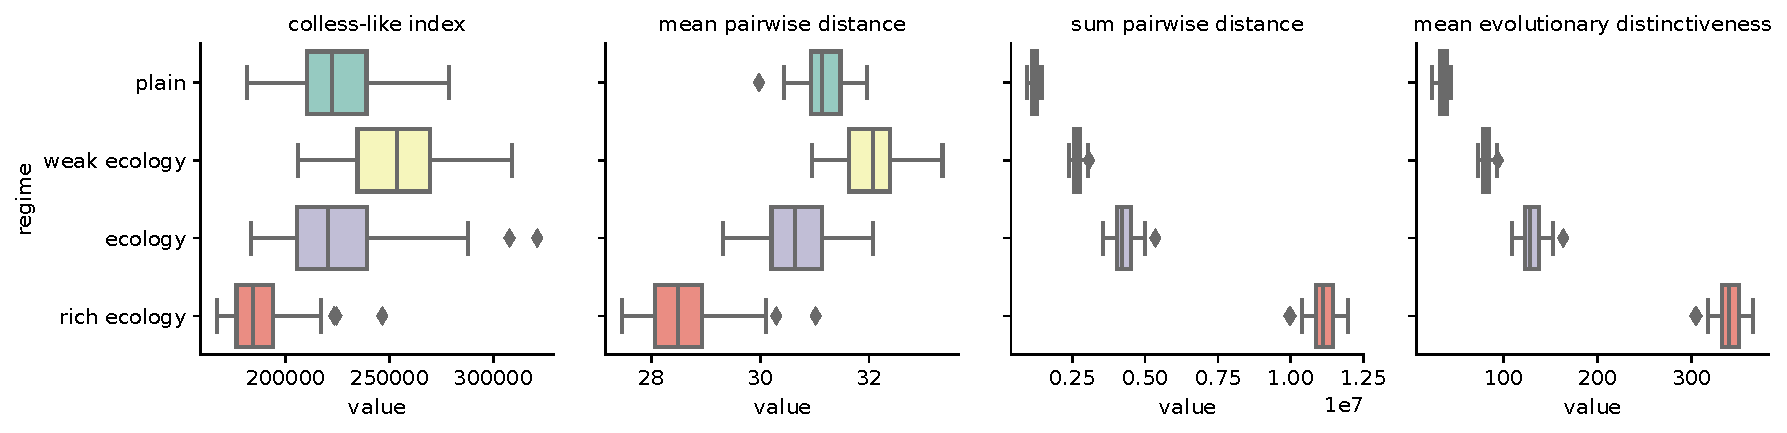
\includegraphics[width=\textwidth]{binder/binder/teeplots/col=phylometric+epoch=7+mut_distn=np.random.standard_normal+nuisance=spatial-structure+viz=boxplot+x=value+y=regime+ext=.pdf}
  \caption{TODO}
  \label{fig:perfect-tree-phylometrics-with-spatial-nuisance}
\end{figure*}


At large scale, digital evolution populations will almost inevitably integrate spatial structure due to practical limitations of distributed computing hardware \citep{ackley2014indefinitely}.
Therefore, understanding the background effects of spatial structure on the phylogenetic signatures of other evolutionary dynamics will be essential to applications of phylogenetic inference in such applications.
For this analysis, we chose to focus on ecological dynamics due to interest in how their relatively weak phylometric signatures would respond to the relatively strong influence of spatial structure.

Figure \ref{fig:perfect-tree-phylometrics-with-spatial-nuisance} summarizes the distribution of surveyed phylometrics under the three surveyed ecological regimes and the control non-ecological regime, all with spatial population structure.
Statistical tests confirmed that each phylometric exhibited significant  variation among these evolutionary regimes (Kruskal-Wallis tests; all $p < 1\times10^{-20}$; $n=50$ per condition; Supplementary Table perfect-tree-phylometrics-with-spatial-nuisance-kruskal).

To explore the nature of this variation, we performed all-pairs comparisons for each phylometric among the four surveyed regimes (Wilcoxon tests with Bonferoni correction; corrected significance threshold $5.26 \times 10^{-4}$; $n=50$ per condition; 24 comparisons per sensitivity analysis configuration; 96 comparisons total; Supplementary Table perfect-tree-phylometrics-with-spatial-nuisance-wilcox).
Like under the spatially unstructured background, ecology drove significant increases and mean evolutionary distinctiveness. 
Unlike the spatially unstructured background, though, ancestor count under ecological conditions sharply exceeded ancestor count under non-ecological conditions.
Ancestor count significantly increased between the 4 niche ecological regimes and the 8 niche ecological regime, as well.
Additionally,  the 8 niche regime significantly decreases mean pairwise distance under under spatially-structured conditions.
This was not the case without spatial structure.

Spatial structure appears to mediate these aspects of ecological phylogenetic structure, they do not appear in its absence.
However, spatial structure mutes the effects of ecology on the Colless-like index.
Only the 8 niche regime significantly decreased this phylometric. 

For these experiments, we again performed a sensitivity analysis over an alternate exponential mutation operator and earlier phylogeny sampling timepoints.
We found the effects of evolutionary conditions on phylometrics to be generally consistent across surveyed conditions (Supplementary Figure \ref{fig:perfect-tree-phylometrics-sensitivity-analysis-with-spatial-nuisance} and Supplementary Tables tab:perfect-tree-phylometrics-with-spatial-nuisance-kruskal and tab:perfect-tree-phylometrics-with-spatial-nuisance-wilcox). 

% . We found significant differences for all metrics except

% epoch 7
% \begin{itemize}
%     \item 4 niche ecology	plain	49	colless like index
% \item weak 4 niche ecology	4 niche ecology	49	num ancestors
% \end{itemize}

% epoch 0
% \begin{itemize}

% \item plain	weak 4 niche ecology	50	colless like index
% \item plain	weak 4 niche ecology	50	mean pairwise distance
% \item weak 4 niche ecology	4 niche ecology	50	num ancestors

% \end{itemize}

% epoch 2
% \begin{itemize}
%     \item weak 4 niche ecology	4 niche ecology	50	num ancestors
% \end{itemize}

% exponential
% \begin{itemize}
%     \item 4 niche ecology	plain	50	colless like index
%     \item 4 niche ecology	plain	50	mean pairwise distance
%     \item 4 niche ecology	weak 4 niche ecology	50	num ancestors
% \end{itemize}


\subsection{Phylometrics with Reconstruction Error Nuisance}

\begin{sidewaysfigure*}
  \centering
  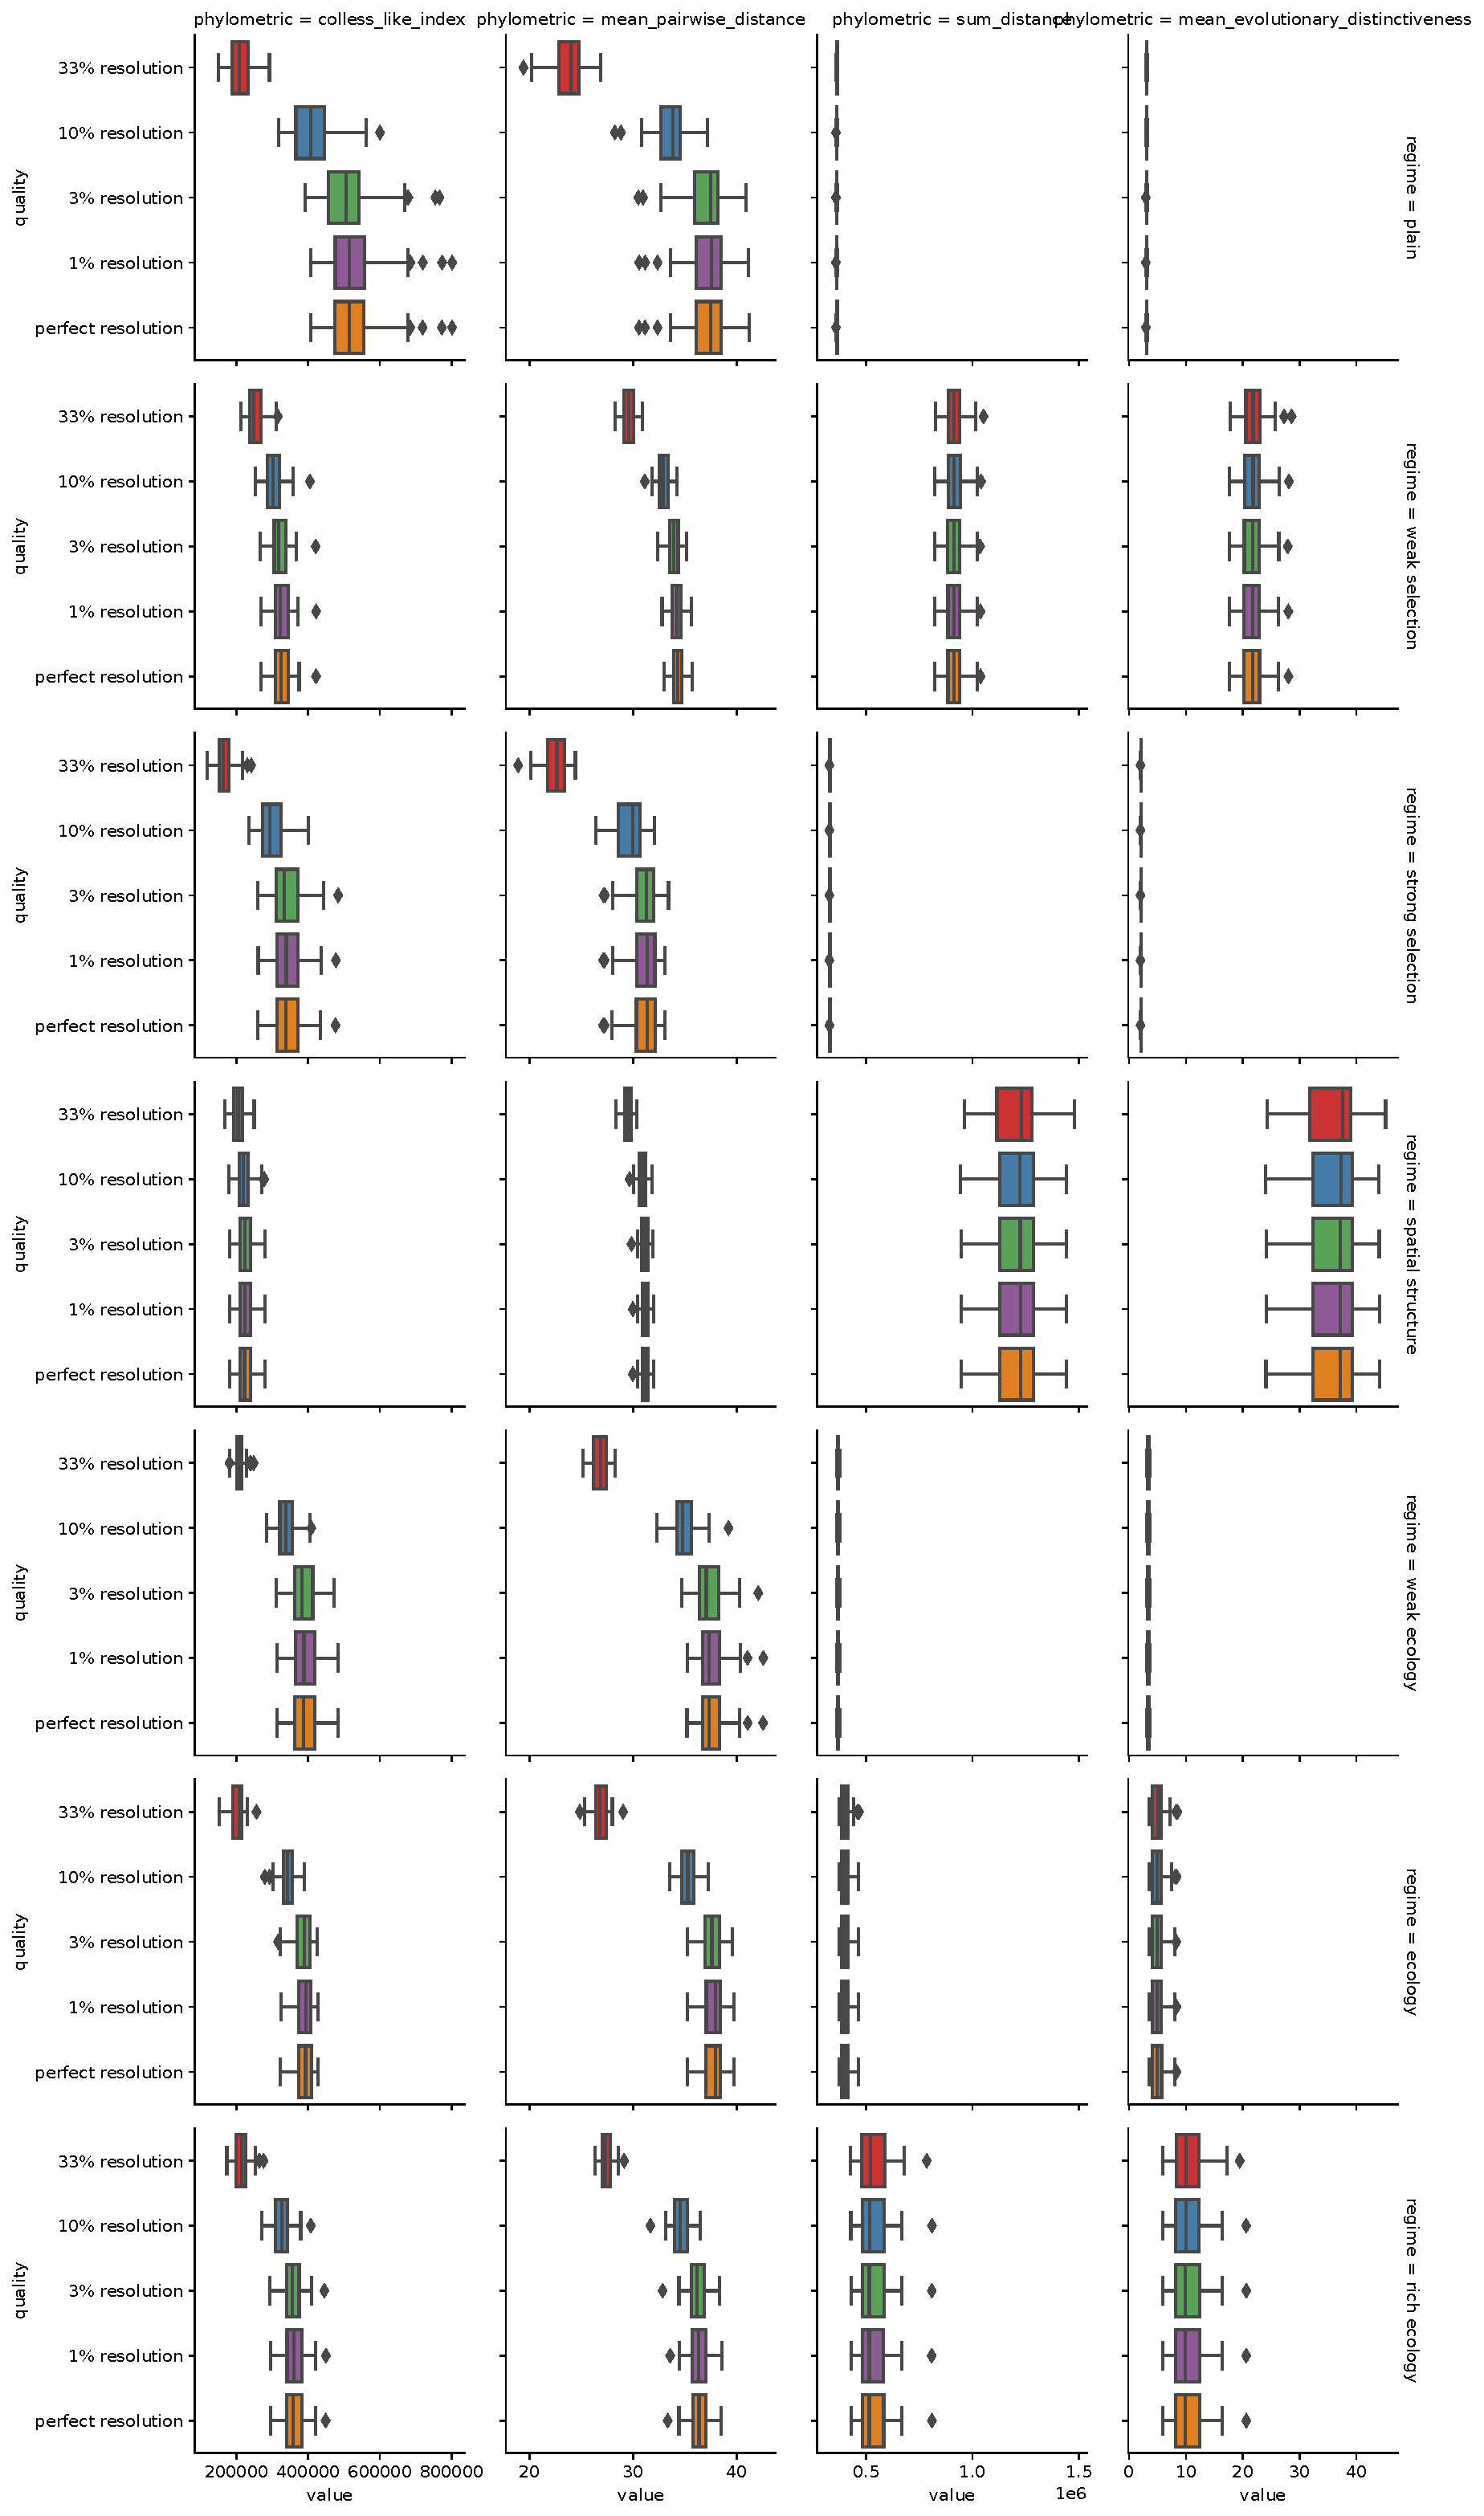
\includegraphics[height=\textwidth,angle=-90,origin=c]{binder/binder/teeplots/col=phylometric+epoch=7+mut_distn=np.random.standard_normal+row=regime+viz=boxplot+x=value+y=quality+ext=.pdf}
  \caption{TODO}
  \label{fig:reconstructed-tree-phylometrics}
\end{sidewaysfigure*}


Shifting from perfect phylogenetic tracking to approxmate phylogentic reconstruction will facilitate efficienct and robust digital evolution simulations at scale, but introduces a complicating factor into phylogenetic analyses: reconstruction error.
Effective phylogenetic analyses will require an understanding potential effects of this error on calculated phylometrics.

figure facet boxplot

STATISTICS: do phylometrics vary by resolution for each regime?
TODO

\begin{figure*}
  \centering
  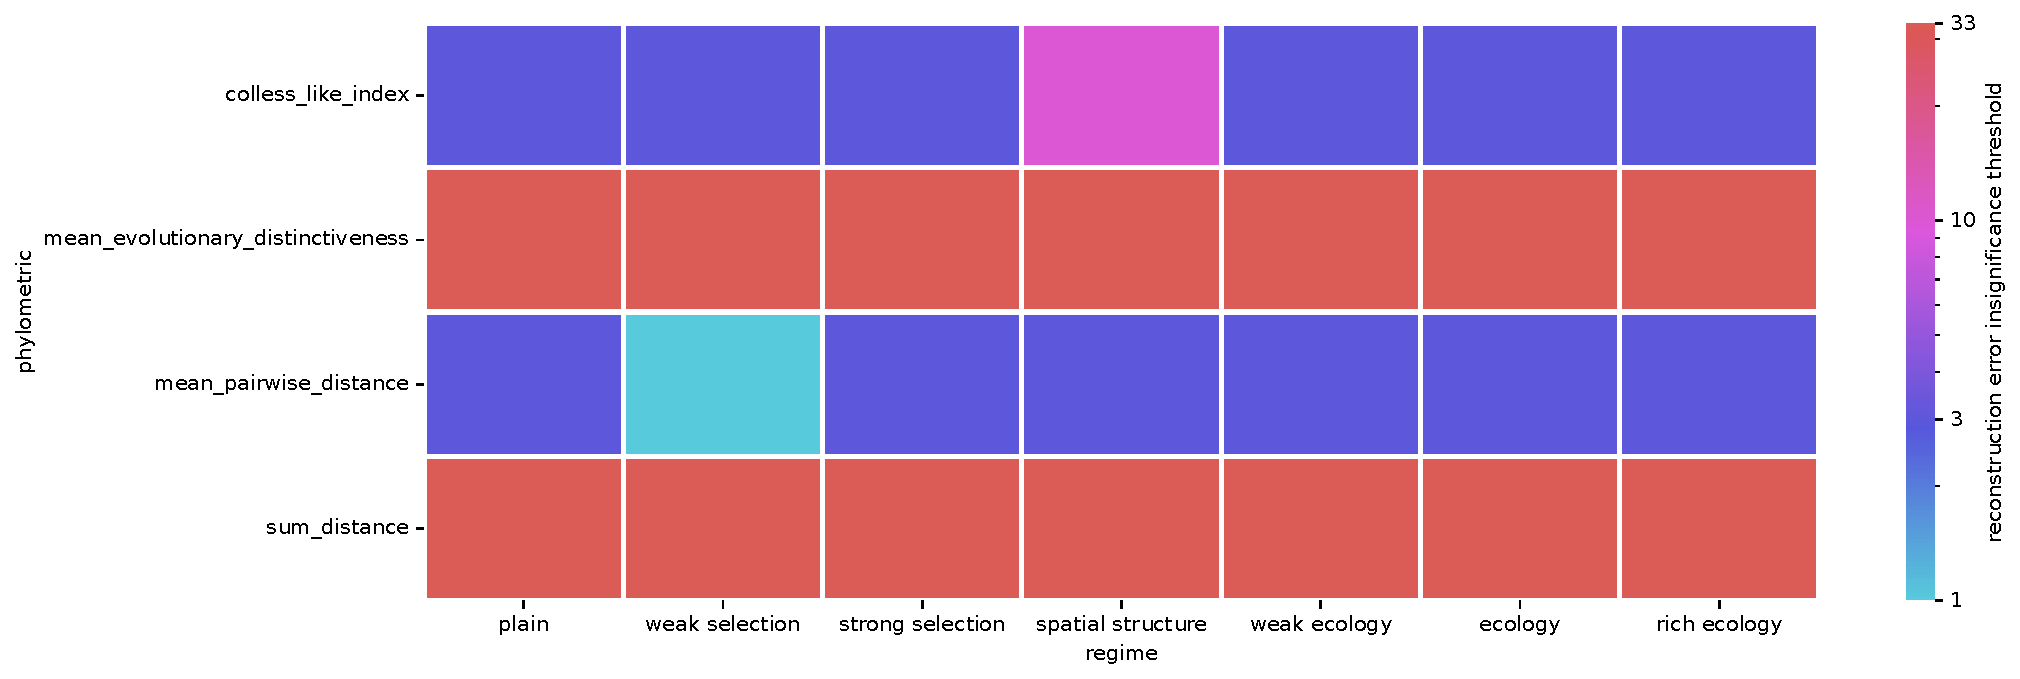
\includegraphics[width=\textwidth]{binder/binder/teeplots/epoch=7+hue=quality-threshold+mut_distn=np.random.standard_normal+viz=heatmap+x=regime+y=phylometric+ext=.pdf}
  \caption{TODO}
  \label{fig:reconstructed-tree-phylometrics-error}
\end{figure*}


Supplementary Figure \ref{fig:reconstructed-tree-phylometrics-error-sensitivity-analysis}.

\subsection{Phylometrics with Spatial Structure and Reconstruction Error Nuisances}

figure facet boxplot
\begin{figure*}
  \centering
  % \begin{noindent}
  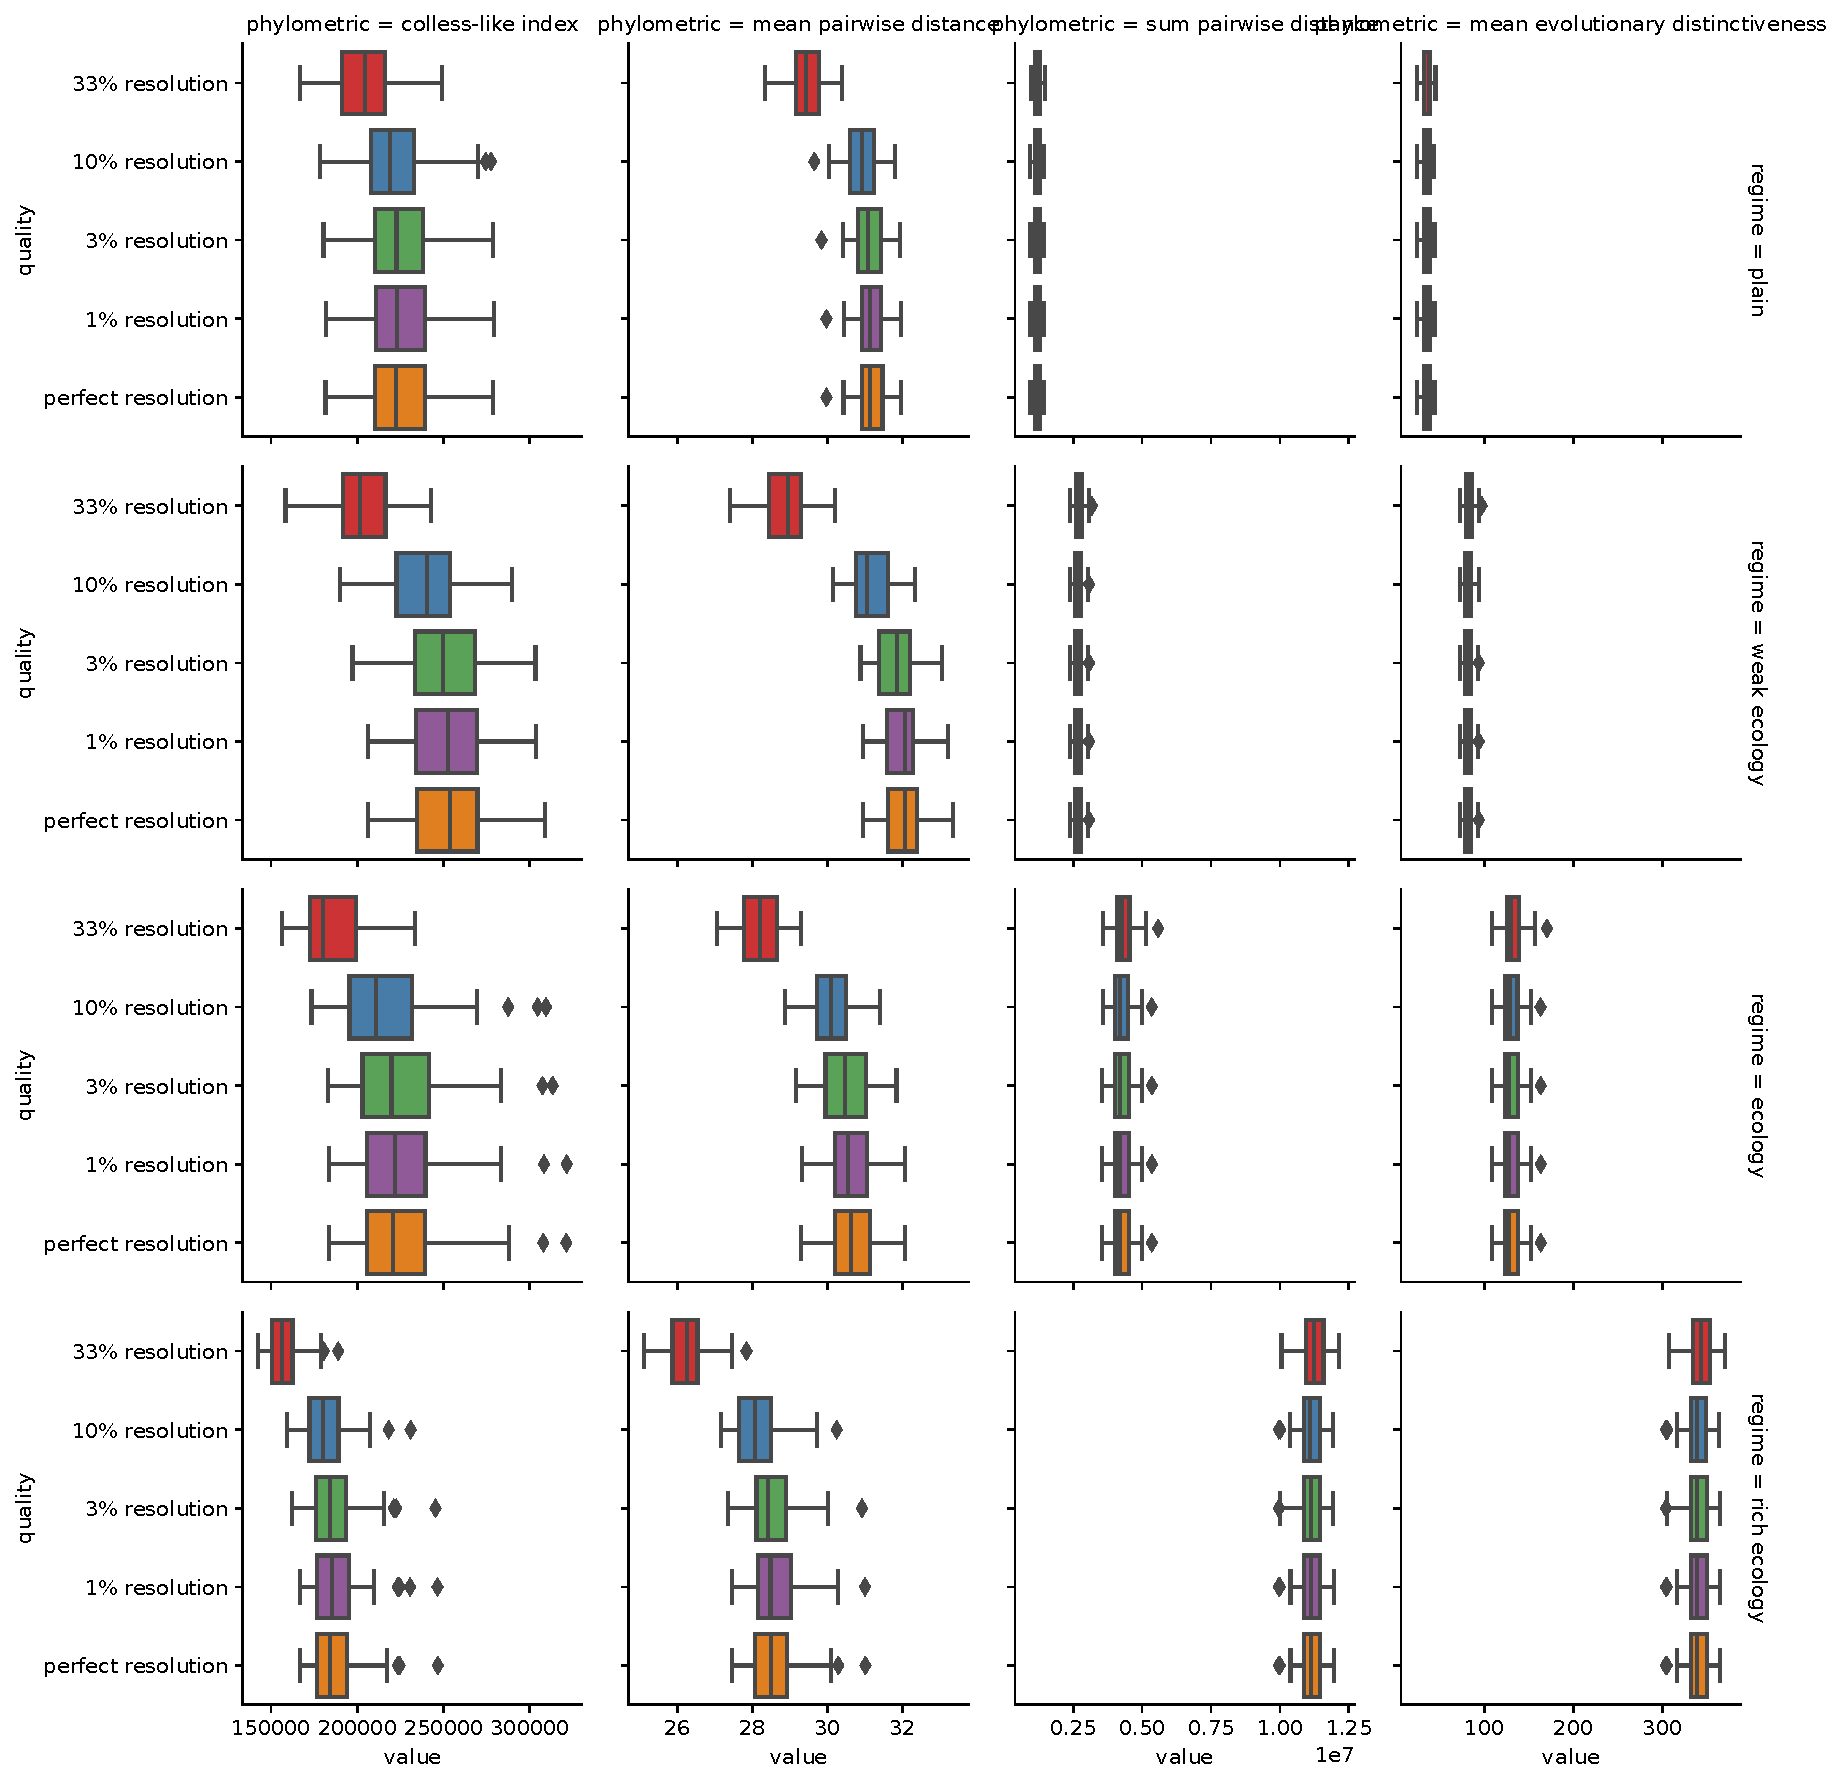
\includegraphics[width=\textwidth]{binder/binder/teeplots/col=phylometric+epoch=7+mut_distn=np.random.standard_normal+nuisance=spatial-structure+row=regime+viz=boxplot+x=value+y=quality+ext=.pdf}
  % \end{noindent}
  \caption{%
    Distributions of phylometrics across surveyed reconstruction fidelities for evolutionary regimes with underlying spatial structure (i.e., 1,024 niches).
    Results are for standard experimental conditions: gaussian mutation distribution at epoch 7 (generation 262,144).
    See Figures \labelcref{fig:reconstructed-tree-phylometrics-with-spatial-nuisance-epoch0,fig:reconstructed-tree-phylometrics-with-spatial-nuisance-epoch2,fig:reconstructed-tree-phylometrics-with-spatial-nuisance-exponential} for results under sensitivity analysis conditions.
    Sample sizes of $n=50$ replicates define each depicted distribution.
  }
  \label{fig:reconstructed-tree-phylometrics-with-spatial-nuisance}
\end{figure*}


STATISTICS: do phylometrics vary by resolution for each regime?
TODO

\begin{figure*}
  \centering
  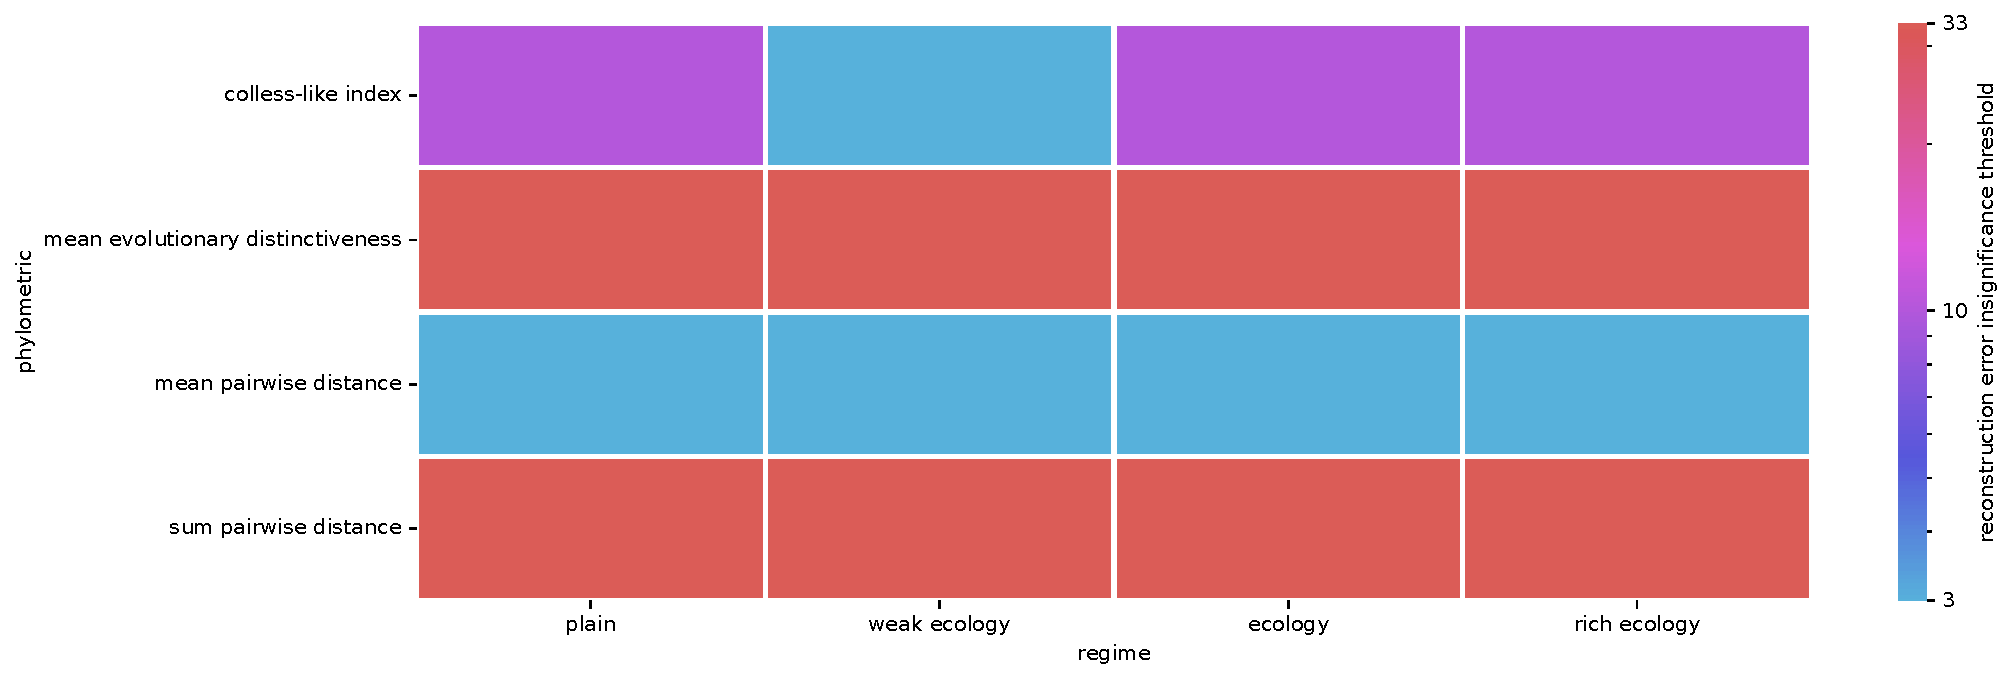
\includegraphics[width=\textwidth]{binder/binder/teeplots/epoch=7+hue=quality-threshold+mut_distn=np.random.standard_normal+nuisance=spatial-structure+viz=heatmap+x=regime+y=phylometric+ext=.pdf}
  \caption{%
    TODO}
  \label{fig:reconstructed-tree-phylometrics-error-spatial-nuisance}
\end{figure*}



\subsection{Tree Reconstruction Quality}

\begin{figure}
  \centering
  \begin{subfigure}[b]{\linewidth}
    \centering
    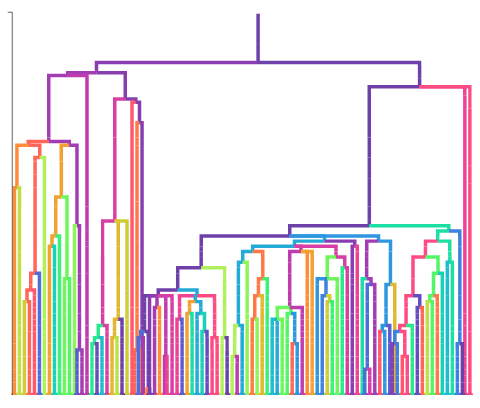
\includegraphics[width=\textwidth, height=0.13\textheight]{img/reference}
    \caption{%
      reference tree}
    \label{fig:plain-perfect-and-reconstruction-phylogenies:reference}
  \end{subfigure}
  \begin{subfigure}[b]{\linewidth}
    \centering
    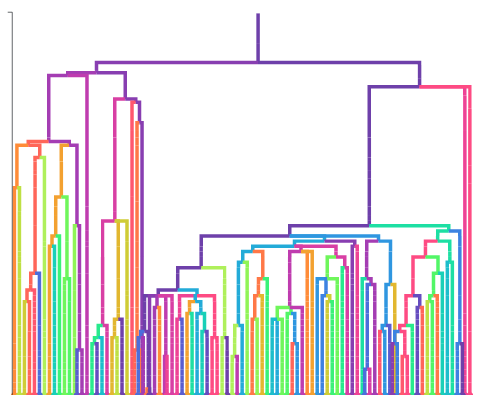
\includegraphics[width=\textwidth, height=0.13\textheight]{img/plain_resolution_100}
    \caption{%
      1\% resolution}
    \label{fig:plain-perfect-and-reconstruction-phylogenies:resolution_100}
  \end{subfigure}
  \begin{subfigure}[b]{\linewidth}
    \centering
    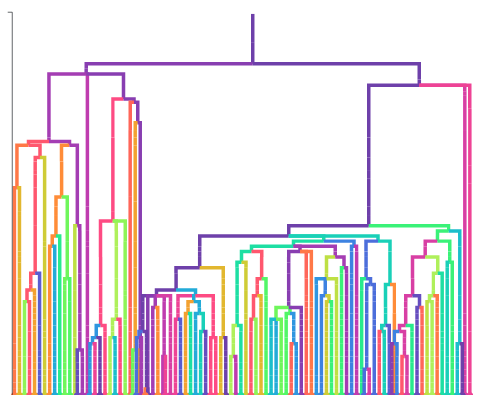
\includegraphics[width=\textwidth, height=0.13\textheight]{img/plain_resolution_30}
    \caption{%
      3\% resolution}
    \label{fig:plain-perfect-and-reconstruction-phylogenies:resolution_30}
  \end{subfigure}
  \begin{subfigure}[b]{\linewidth}
    \centering
    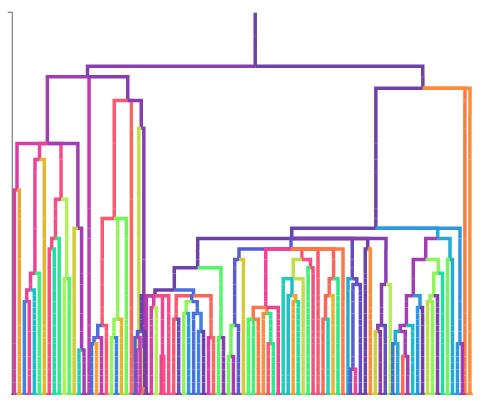
\includegraphics[width=\textwidth, height=0.13\textheight]{img/plain_resolution_10}
    \caption{%
      10\% resolution}
    \label{fig:plain-perfect-and-reconstruction-phylogenies:resolution_10}
  \end{subfigure}
  % \begin{noindent}
  \begin{subfigure}[b]{\linewidth}
    \centering
    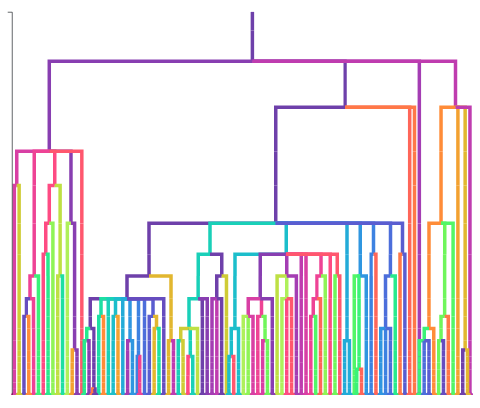
\includegraphics[width=\textwidth, height=0.13\textheight]{img/plain_resolution_3} \caption{%
      33\% resolution}
    \label{fig:plain-perfect-and-reconstruction-phylogenies:resolution_3}
  \end{subfigure}
  % \end{noindent}
  \caption{%
  \textbf{Comparison of phylogeny reconstructions across different hereditary stratigraphy resolutions in the plain evolutionary regime.}
    To maintain visual legibility, these trees contain the same sub-sample of 100 leaf nodes out of the 32,768 in the full trees.
    Sub-figures are arranged from top to bottom in coarsening order of reconstruction resolution.
    Taxon and branch color coding is consistent across subpanels.
    Visit \url{mmore500.com/hstrat-evolutionary-inference/} for mouseover-based highlighting of corresponding clades between reconstructions and reference.
  }
  \label{fig:plain-perfect-and-reconstruction-phylogenies}
\end{figure}


mean/std/max
plain	1% resolution	epoch=7+mut_distn=np.random.standard_normal	-2.10425894221959E-14	1.50722607904943E-16	-2.08295182385988E-14
plain	10% resolution	epoch=7+mut_distn=np.random.standard_normal	-2.10469692847644E-14	1.55963069867711E-16	-2.08314605325639E-14
plain	3% resolution	epoch=7+mut_distn=np.random.standard_normal	-2.10620443554657E-14	1.51986960038139E-16	-2.08462322970661E-14
plain	33% resolution	epoch=7+mut_distn=np.random.standard_normal	-2.10637937229546E-14	1.4397013470276E-16	-2.08299428020224E-14


spatial structure	1% resolution	epoch=7+mut_distn=np.random.standard_normal	7.81849234344143E-07	4.14508890707294E-06	2.82106734844714E-05
spatial structure	10% resolution	epoch=7+mut_distn=np.random.standard_normal	0.00275016417111772	0.0106125775395443	0.0533132541036293
spatial structure	3% resolution	epoch=7+mut_distn=np.random.standard_normal	0.000857215705953448	0.00540569979603497	0.0380983817532154
spatial structure	33% resolution	epoch=7+mut_distn=np.random.standard_normal	0.00763527603510759	0.0149106058655545	0.0584668625701303

mean, std, and max quartet error summary statistics for each reconstruction regime/resolution are provided in Supplementary Table TODO


KRUSKAL WALLIS by resolution
% 38 	50 	4 	quartet_distance 	17.612788 	5.285933e-04 	spatial structure 	7 	np.random.standard_normal
%
% 31 	50 	4 	quartet_distance 	11.319749 	1.011675e-02 	spatial structure 	7 	np.random.exponential
%
% 23 	50 	4 	quartet_distance 	9.640107 	2.188663e-02 	plain 	2 	np.random.standard_normal
% 24 	50 	4 	quartet_distance 	148.020119 	7.044412e-32 	spatial structure 	2
% np.random.standard_normal
%
% 50 	4 	quartet_distance 	100.829421 	1.030737e-21 	weak selection 	0 	np.random.standard_normal

Full statistical results are in Supplementary Table TODO

KRUSKAL WALLIS by regime for each resolution

SIGNIFICANT $p < 0.02$ over all regimes for all resolutions and all sensitivity analysis variables
